\section{Software: Freefem++}
\label{sec:Freefem++:software}



\begin{table}[h!]
    \centering
    { \setlength{\parindent}{0pt}
    \def\arraystretch{1.25}
    \arrayrulecolor{numpexgray}
    {\fontsize{9}{11}\selectfont
    \begin{tabular}{!{\color{numpexgray}\vrule}p{.4\textwidth}!{\color{numpexgray}\vrule}p{.6\textwidth}!{\color{numpexgray}\vrule}}
        \rowcolor{numpexgray}{\rule{0pt}{2.5ex}\color{white}\bf Field} & {\rule{0pt}{2.5ex}\color{white}\bf Details} \\
        \rowcolor{white}\textbf{Consortium} & \begin{tabular}{l}
Sorbonne U\\
\end{tabular} \\
        \rowcolor{numpexlightergray}\textbf{Exa-MA Partners} & \begin{tabular}{l}
Inria PARIS\\
Sorbonne U\\
\end{tabular} \\
        \rowcolor{white}\textbf{Contact Emails} & \begin{tabular}{l}
frederic.hecht@sorbonne-universite.fr\\
pierre-henri.tournier@sorbonne-universite.fr\\
pierre.jolivet@sorbonne-universite.fr\\
\end{tabular} \\
        \rowcolor{numpexlightergray}\textbf{Supported Architectures} & \begin{tabular}{l}
CPU Only\\
\end{tabular} \\
        \rowcolor{white}\textbf{Repository} & \href{https://github.com/FreeFem/FreeFem-sources}{https://github.com/FreeFem/FreeFem-sources} \\
        \rowcolor{numpexlightergray}\textbf{License} & \begin{tabular}{l}
OSS:: LGPL v*\\
\end{tabular} \\
        \rowcolor{white}\textbf{Bottlenecks roadmap} & \begin{tabular}{l}
B10 - Scientific Productivity\\
B11 - Reproducibility and Replicability of Computation\\
B6 - Data Management\\
B7 - Exascale Algorithms\\
\end{tabular} \\
        \bottomrule
    \end{tabular}
    }}
    \caption{Freefem++ Information}
\end{table}

\subsection{Software summary}
\label{sec:Freefem++:summary}
FreeFEM is a free open-source software developed at Laboratoire Jacques-Louis Lions and designed for one- to three-dimensional multi-physics simulations. It has been continuously developed since 1992 and has an active community of users; the community forum averages around 25 discussion topics per month. The FreeFEM source code is hosted on Github, with the repository having (at time of writing) 764 stars and 189 forks and 1500 binary downloads per month on average. FreeFEM leverages the strengh of the team in numerical analysis and scientific computing, with finite element methods (FEM), boundary element methods (BEM) and domain decomposition (DD) methods implemented to a high level. It works on Linux, MacOS and Windows and can run in various architectures from cell phones to national supercomputers. \\

FreeFEM embeds a high-level user-friendly Domain Specific Language (DSL), which allows users with minimal programming knowledge to describe and solve their problems with a few lines of code. Its main objective is to provide easy access to distributed parallel simulations and solvers while hiding technical programming difficulties from the user. FreeFEM is written in C++ for speed, and features easy custom extensions through dynamically-loaded plugins.\\
On the one hand, FreeFEM’s DSL allows users to easily define and manipulate high-level notions such as variational forms, meshes, and FEM or BEM spaces; on the other hand, the user can also access the underlying data structures and linear algebra (i.e., FreeFEM is not a “black box" that cannot be opened). It allows rapid multiphysics prototyping ; the resulting scripts are  close to their mathematical counterparts. The abstraction of the DSL reduces the gap between mathematical objects and their numerical and practical implementation. As an illustration, below is a sample script setting up and solving a 2D acoustic scattering problem:

\begin{figure}[h!]
\begin{minipage}{.45\textwidth}
\begin{center}
Code\\[1em]

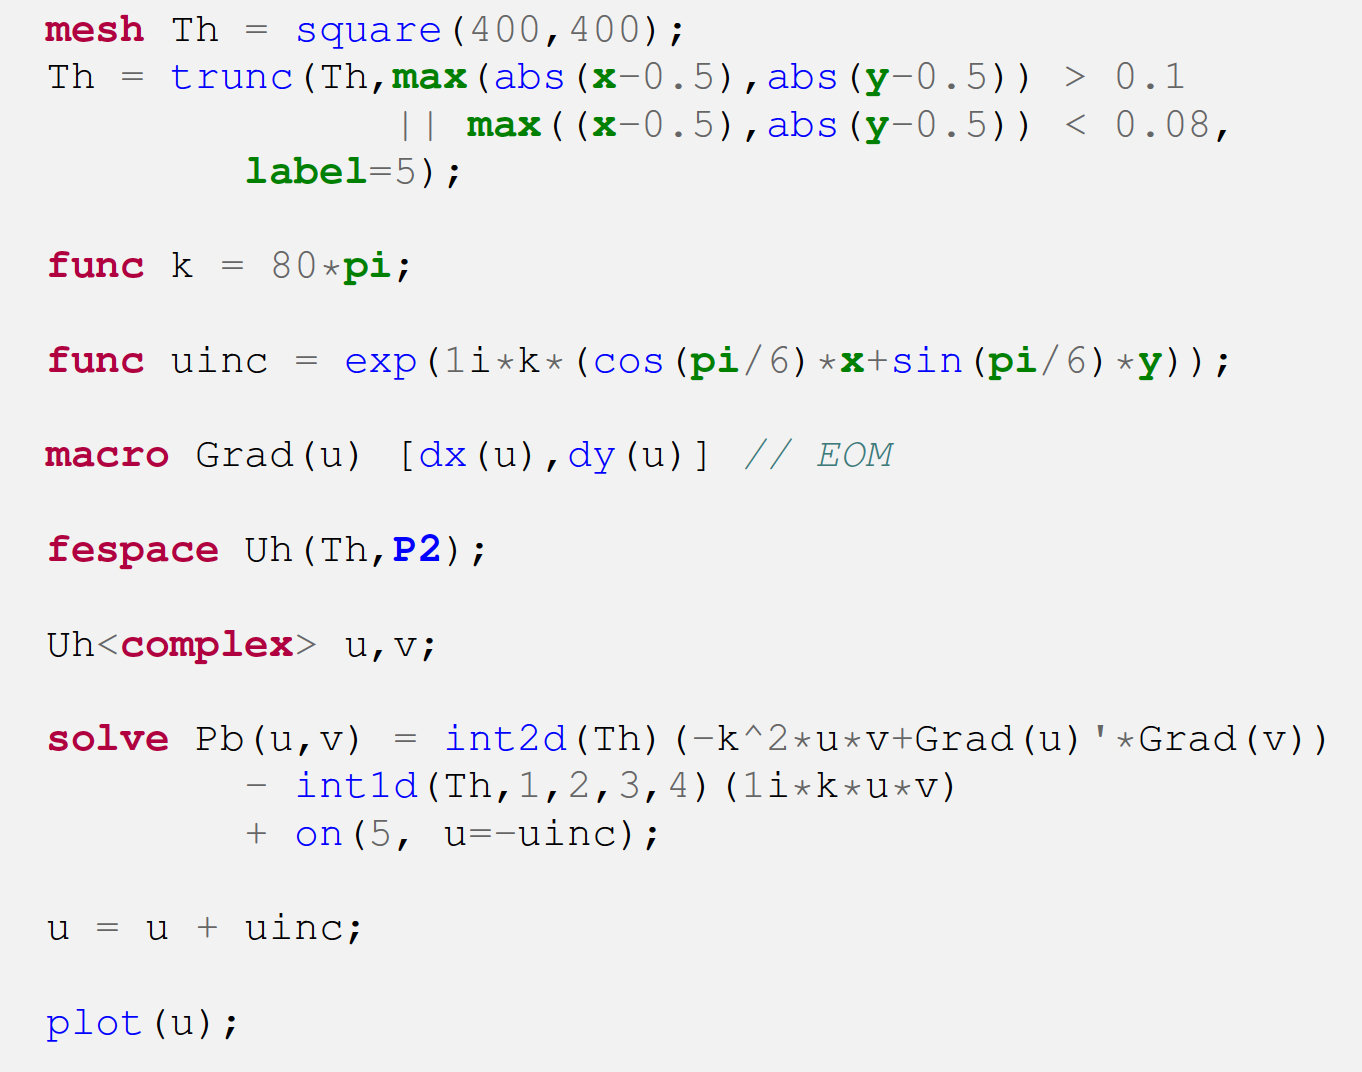
\includegraphics[height=6cm]{graphics/freefempp/samplecode.png}\end{center}
\end{minipage}
\hfill
\begin{minipage}{.45\textwidth}
\begin{center}
Output\\[1em]

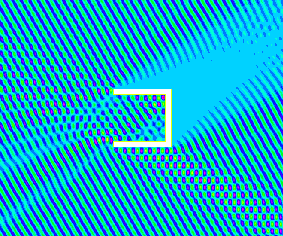
\includegraphics[height=6cm]{graphics/freefempp/sampleplot.pdf}
\end{center}
\end{minipage}
\caption{Sample FreeFEM code solving a 2D acoustic scattering problem by a rectangular cavity.}
\end{figure}

The DSL allows the end user to easily implement their own physics modules using the provided FreeFEM language. Numerous physics are pre-built: Incompressible Navier-Stokes (using the P1-P2 Taylor Hood element), Lamé equations (linear elasticity), Neo-Hookean, Mooney-Rivlin (nonlinear elasticity), Thermal diffusion, Thermal convection, Thermal radiation, Magnetostatics, Electrostatics, Fluid-structure interaction (FSI),...\\
FreeFEM supports 1D (curvilinear), 2D (surface) and 3D simplicial meshes. It embeds its own 2D internal mesher and is compatible with powerful open-source mesh and visualization software such as Tetgen, Gmsh, Mmg, ParMmg and ParaView.\\

FreeFEM is interfaced with state of the art parallel solvers and libraries such as

\begin{itemize}
\item the HPDDM library, which contains optimized C++ MPI-parallel implementation of the latest domain-decomposition methods,
\item the HTOOL library, a high-performance parallel library implementing domain-decomposition solvers and Hierarchical matrix (H-matrix)
compression for BEM operators using hybrid OpenMP-MPI parallelism
\item the PETSc library (Portable, Extensible Toolkit for Scientific Computation), giving access to a wide variety of solvers in one easy-to-use toolbox. 
\end{itemize}

Being developed hand-in-hand with the team's research in scientific computing, FreeFEM benefits from the fast integration of the latest state of the art research developments in particular regarding fast and robust parallel linear solvers, allowing the software to remain at the forefront in the scientific community and contribute to important applications in various fields such as health, medical imaging, earth science, climatology, computational fluid dynamics, quantum mechanics, finance, ...

\subsection{Purpose}
\label{sec:Freefem++:purpose}

FreeFEM aims to bring scientific computing to everyone, allowing the user to easily set up and perform multiphysics numerical simulations while enjoying the performance and scalability of state of the art robust parallel solvers.

\subsection{Programming and Computational Environment}
\label{sec::Freefem++:environment_capabilities}


Table~\ref{tab:Freefem++:env} summarizes these aspects for Freefem++, providing a  view of its programming and computational capabilities.

\begin{table}[h!]
    \centering
    {
    \setlength{\parindent}{0pt}
    \def\arraystretch{1.25}
    \arrayrulecolor{numpexgray}
    {\fontsize{9}{11}\selectfont
    \begin{tabular}{lp{.3\textwidth}p{.5\textwidth}}
        \rowcolor{numpexgray}{\rule{0pt}{2.5ex}\color{white}\bf Category}  & {\rule{0pt}{2.5ex}\color{white}\bf Details} & {\rule{0pt}{2.5ex}\color{white}\bf Description}\\
        \rowcolor{white}Languages  & \begin{tabular}{l}
C++\\
\end{tabular} & FreeFEM is written in C++ for speed and allows the user to easily add features in the language through dynamically-loaded C++ plugins. FreeFEM mainly uses the C++14 standard. \\
        \rowcolor{numpexlightergray}Parallelism  & \begin{tabular}{l}
MPI\\
\end{tabular} & FreeFEM relies on MPI for distributed memory parallelism. FreeFEM provides a rich and robust interface to state of the art MPI-parallel solver libraries such as PETSc and HPDDM. The user can also define and manage their own distributed parallel data structures thanks to FreeFEM's interface to MPI in the DSL.\\
        \rowcolor{white}Data Formats  & \begin{tabular}{l}
Gmsh and associated formats\\
HDF5\\
VTK\\
in-house format\\
\end{tabular} & FreeFEM supports various standard mesh and data formats for I/O.\\
        \rowcolor{numpexlightergray}Resilience  & \begin{tabular}{l}
None\\
\end{tabular} & FreeFEM does not currently implement resilience functionalities such as fault tolerance or recovery mechanisms.\\
        \rowcolor{white}DevOps & \begin{tabular}{l}
Continuous Integration\\
\end{tabular} & FreeFEM is maintained on GitHub. We are in the process of switching frameworks to use GitHub Actions workflows for Continuous Integration. FreeFEM uses standard development workflows using develop and feature branches ; PRs are reviewed before being merged into the develop branch. The develop branch is merged into master for each software release.\\
        \rowcolor{numpexlightergray}Packaging  & \begin{tabular}{l}
Ubuntu\\
Spack\\
GUIX-HPC\\
\end{tabular} & Software packaging and distribution.\\
        \rowcolor{white}Testing  & \begin{tabular}{l}
Unit\\
Validation\\
\end{tabular} & FreeFEM includes a test suite of more then 600 examples extensively testing and validating the features of the software, both in sequential and parallel settings.\\
        \rowcolor{numpexlightergray}Containerization  & \begin{tabular}{l}
Docker\\
\end{tabular} & Container technologies used to package and deploy the software.\\
        \rowcolor{white}Interfaces  & \begin{tabular}{l}
tetgen\\
MMG/ParMMG\\
MUMPS\\
HPDDM\\
PETSc\\
HTOOL\\
Scotch\\
Metis/ParMetis\\
IPOPT\\

\end{tabular} & FreeFEM interfaces with various software and libraries for mesh generation and mesh adaptation (tetgen/MMG/ParMMG), partitioning(Scotch/Metis/ParMetis), low-rank compression(HTOOL), solvers(MUMPS/HPDDM/PETSc), optimization(IPOPT), ...  \\
        \bottomrule
    \end{tabular}
    }}
    \caption{Freefem++ programming and computational environment}
\label{tab:Freefem++:env}
\end{table}



\subsection{Mathematics}
\label{sec:Freefem++:mathematics}

FreeFEM implements both finite element methods (FEM) and boundary element methods (BEM) for the solution of partial differential equations (PDEs) in complex geometries. It uses various mathematically sound numerical algorithms to enhance the accuracy and speed of the simulations, from metric-based adaptive mesh refinement to provably robust multilevel domain decomposition solvers.


\subsection{Relevant Publications}
\label{sec:Freefem++:publications}

\begin{description}
\item[\fullcite{hecht_new_2012}] This is a short presentation of the capabilities of the software. The documentation is available online at \url{https://doc.freefem.org}.

{TOCITE Mathematics and Finite Element Discretizations of Incompressible Navier-Stokes Flows} This self-contained book provides a thorough theoretical study of finite element methods for solving incompressible Navier-Stokes equations. It focuses on efficient and widely used finite element methods that are well adapted to large-scale simulations. In this revised and expanded edition of Girault and Raviart's 1986 textbook Finite Element Methods for Navier-Stokes Equations, readers will find rigorous proof of stability and convergence, analysis of practical algorithms, and a stand-alone chapter on finite element methods that is applicable to a large range of PDEs. The book also covers a variety of numerical algorithms used in the computer implementation of Navier-Stokes equations and numerical experiments.

{TOCITE An Introduction to Domain Decomposition Methods: Algorithms, Theory, and Parallel Implementation} The purpose of this book is to offer an overview of the most popular domain decomposition methods for partial differential equations (PDEs). The authors present all popular algorithms, both at the PDE level and at the discrete level in terms of matrices, along with systematic FreeFEM scripts for sequential implementation as well as some parallel scripts.

{TOCITE A GenEO Domain Decomposition method for Saddle Point problems} This paper introduces an adaptive element-based domain decomposition (DD) method for solving saddle point problems defined as a block two by two matrix. The algorithm does not require any knowledge of the constrained space. The design of the adaptive coarse space extends the GenEO theory to saddle point problems. Numerical results on three dimensional elasticity problems for steel-rubber structures are shown for up to one billion degrees of freedom.

{TOCITE An 89-line code for geometrically nonlinear topology optimization written in FreeFEM} This paper presents an 89-line code for nonlinear topology optimization written in FreeFEM based on the popular SIMP (solid isotropic material with penalization) method. Excluding thirteen lines which are used for explanation, only 76 lines are needed for the initialization of the design parameters, nonlinear finite element analysis, sensitivity calculation, and updated design variables. Different design problems can be solved by modifying several lines in the proposed program.

{TOCITE PDE-constrained optimization within FreeFEM} This book is aimed at students and researchers who want to learn how to efficiently solve constrained optimization problems involving partial differential equations (PDE) using the FreeFEM software.

{TOCITE Numerical Modeling and High-Speed Parallel Computing: New Perspectives on Tomographic Microwave Imaging for Brain Stroke Detection and Monitoring} This paper deals with microwave tomography for brain stroke imaging using state-of-the-art numerical modeling and massively parallel computing. It includes the accurate modeling of a whole-microwave measurement system. The inverse problem is solved by a gradient based L-BFGS minimization algorithm. The successive solution of the direct problem in the optimization loop is accelerated using an Optimized Restricted Additive Schwarz (ORAS) preconditioner.

{TOCITE Parallel finite-element codes for the simulation of two-dimensional and three-dimensional solid-liquid phase-change systems with natural convection} This work presents a FreeFEM Toolbox for the parallel computing of two- or three-dimensional liquid-solid phase-change systems involving natural convection. Parallel 2D and 3D computations of benchmark cases of increasing difficulty are presented: natural convection of air, natural convection of water, melting or solidification of a phase-change material, water freezing. For each case, careful validations are provided and the performance of the code is assessed. 

{TOCITE Three-dimensional finite-difference finite-element frequency-domain wave simulation with multi-level optimized additive Schwarz domain-decomposition preconditioner: A tool for FWI of sparse node datasets} In seismic imaging, efficient frequency-domain full-waveform inversion (FWI) of long-offset node data can be designed with a few discrete frequencies, which lead to modest data volumes to be managed during the inversion process. This requires the solution of large and sparse linear indefinite systems for each frequency with multiple right-hand sides (RHSs). Here we investigate Optimized Restricted Additive Schwarz (ORAS) preconditioners with Robin or Perfectly Matched Layer (PML) interface conditions. Multiple sources are processed in groups with a pseudo-block method. The accuracy, computational cost and scalability of the solver are assessed against several realistic benchmarks.

{TOCITE Three-dimensional topology optimization of a fluid-structure system using body-fitted mesh adaption based on the level-set method} This paper presents a new framework for the two- and three-dimensional topology optimization of the weakly-coupled fluid-structure system. The proposed design methodology uses a reaction-diffusion equation for updating the level-set function based on the topological sensitivity. The performance of the methodology is demonstrated by solving three different optimization problems: compliance, power dissipation, and fluid-structure interaction. For comparison and for assessing the various techniques, the designs are benchmarked against state-of-the-art works followed by showcasing a variety of practical engineering design examples.

{TOCITE Geometrical shape optimization in fluid mechanics using FreeFem++} This paper presents simple and robust numerical methods for two-dimensional geometrical shape optimization problems, in the context of viscous flows driven by the stationary Navier-Stokes equations at low Reynolds number. Several pedagogical examples are discussed. The corresponding program is written in the FreeFem++ environment, and it is freely available. Its chief features are carefully presented, so that it can easily be handled and elaborated upon to deal with different, or more complex physical situations.

{TOCITE Radiative transfer for variable three-dimensional atmospheres} To study the temperature in a gas subjected to electromagnetic radiations, one may use the Radiative Transfer equations coupled with the Navier-Stokes equations. The problem has 7 dimensions but can be simplified to a small number of integro-differential equations in 3 dimensions. This work presents the method and its numerical implementation using a Hierarchical matrix compression scheme, using FreeFEM and HTOOL. Applications to the temperature in the French Chamonix valley are presented with and without snow or cloud and with a variable absorption coefficient taken from the Gemini measurements. The software is precise enough to assert temperature differences due to increased absorption in the vibrational frequency subrange of greenhouse gases.

{TOCITE A finite element toolbox for the Bogoliubov-de Gennes stability analysis of Bose-Einstein condensates} This work presents a FreeFEM finite element toolbox for the computation of Bogoliubov-de Gennes modes used to assess the linear stability of stationary solutions of the Gross-Pitaevskii (GP) equation. Applications concern one (single GP equation) or two-component (a system of coupled GP equations) Bose-Einstein condensates in one, two and three dimensions of space. Programs are validated through comparisons with known theoretical results for simple cases and numerical results reported in the literature.
\end{description}

\subsection{Acknowledgements}
\label{sec::Freefem++:acknowledgements}

The software has been developed with the support of the following funding agencies, institutions and private companies: 

\begin{itemize}
\item Sorbonne Université
\item University of Rouen
\item INRIA
\item ANR
\item Airthium company
\end{itemize}